\documentclass{standalone}
\usepackage{amsfonts,amsmath,amssymb}
\usepackage[slovene]{babel}
\usepackage[utf8]{inputenc}
\usepackage[T1]{fontenc}
  
\usepackage{tikz, verbatim}
\usepackage{pgfplots}
\usetikzlibrary{arrows.meta, calc, positioning, automata}

\newcommand{\subdiv}[3] {
\draw ($ 0.5*#2 + 0.5*#3 $) -- #1;
\draw ($ 0.5*#1 + 0.5*#3 $) -- #2;
\draw ($ 0.5*#1 + 0.5*#2 $) -- #3;
}
\begin{document}

	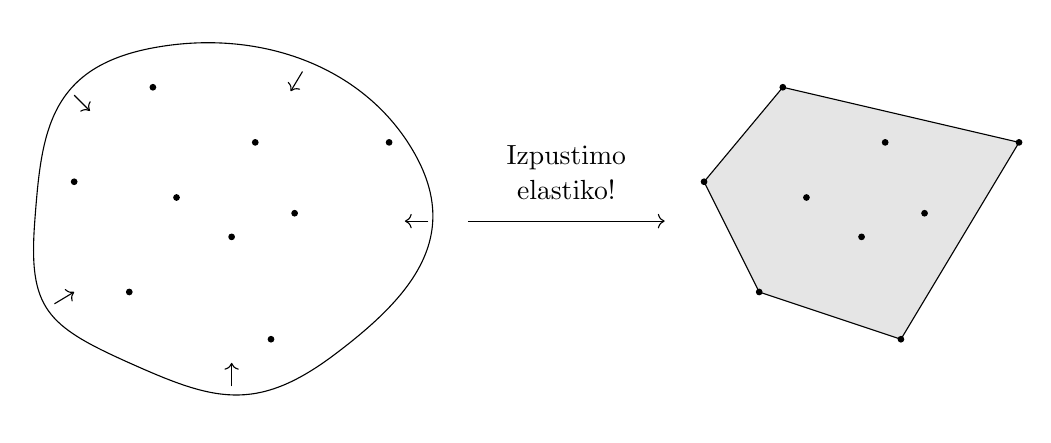
\begin{tikzpicture}
% ####################   elastika    ####################
		\draw plot [smooth cycle, tension = 1] coordinates {(-1, 2.2) (-2.5, 0) (-1.3, -1.8) (1.3, -1.7) (2.3, 0.9)};
% ####################   puščice, ki označujejo, da se elastika skrči    ####################
		\draw[->] (-2, 1.6) -- (-1.8, 1.4);
		\draw[->] (-2.25, -1.05) -- (-2, -0.9);
		\draw[->] (0, -2.1) -- (0, -1.8);
		\draw[->] (2.5, 0) -- (2.2, 0);
		\draw[->] (0.9, 1.9) -- (0.75, 1.65);
% ####################   robne točke, ki jih omejuje elastika    ####################
		\filldraw[black] (-1, 1.7) circle (1pt);
		\filldraw[black] (-1.3, -0.9) circle (1pt);
		\filldraw[black] (2, 1) circle (1pt);
		\filldraw[black] (-2, 0.5) circle (1pt);
		\filldraw[black] (0.5, -1.5) circle (1pt);
% ####################   notranje točke, ki jih omejuje elastika    ####################
		\filldraw[black] (-0.7, 0.3) circle (1pt);
		\filldraw[black] (0.3, 1) circle (1pt);
		\filldraw[black] (0, -0.2) circle (1pt);
		\filldraw[black] (0.8, 0.1) circle (1pt);
% ####################   oblika elastike, ko jo izpustimo    ####################
		\filldraw[fill=gray!20] (7, 1.7) -- (6, 0.5)  -- (6.7, -0.9)  -- (8.5, -1.5) -- (10, 1) -- cycle;
% ####################   robne točke, na katerih je napeta elastika    ####################
		\filldraw (7, 1.7) circle (1pt);
		\filldraw (6.7, -0.9) circle (1pt);
		\filldraw (10, 1) circle (1pt);
		\filldraw (6, 0.5) circle (1pt);
		\filldraw (8.5, -1.5) circle (1pt);
% ####################   notranje točke    ####################
		\filldraw[black] (7.3, 0.3) circle (1pt);
		\filldraw[black] (8.3, 1) circle (1pt);
		\filldraw[black] (8, -0.2) circle (1pt);
		\filldraw[black] (8.8, 0.1) circle (1pt);
% ####################   puščice    ####################
		\draw[->] (3, 0) -- (5.5,0);
		\draw (4.25, 0.8) node {Izpustimo};
		\draw (4.25, 0.4) node {elastiko!};
	\end{tikzpicture}
	
\end{document}